% Options for packages loaded elsewhere
\PassOptionsToPackage{unicode}{hyperref}
\PassOptionsToPackage{hyphens}{url}
%
\documentclass[
]{article}
\usepackage{amsmath,amssymb}
\usepackage{lmodern}
\usepackage{iftex}
\ifPDFTeX
  \usepackage[T1]{fontenc}
  \usepackage[utf8]{inputenc}
  \usepackage{textcomp} % provide euro and other symbols
\else % if luatex or xetex
  \usepackage{unicode-math}
  \defaultfontfeatures{Scale=MatchLowercase}
  \defaultfontfeatures[\rmfamily]{Ligatures=TeX,Scale=1}
\fi
% Use upquote if available, for straight quotes in verbatim environments
\IfFileExists{upquote.sty}{\usepackage{upquote}}{}
\IfFileExists{microtype.sty}{% use microtype if available
  \usepackage[]{microtype}
  \UseMicrotypeSet[protrusion]{basicmath} % disable protrusion for tt fonts
}{}
\makeatletter
\@ifundefined{KOMAClassName}{% if non-KOMA class
  \IfFileExists{parskip.sty}{%
    \usepackage{parskip}
  }{% else
    \setlength{\parindent}{0pt}
    \setlength{\parskip}{6pt plus 2pt minus 1pt}}
}{% if KOMA class
  \KOMAoptions{parskip=half}}
\makeatother
\usepackage{xcolor}
\usepackage[margin=1in]{geometry}
\usepackage{longtable,booktabs,array}
\usepackage{calc} % for calculating minipage widths
% Correct order of tables after \paragraph or \subparagraph
\usepackage{etoolbox}
\makeatletter
\patchcmd\longtable{\par}{\if@noskipsec\mbox{}\fi\par}{}{}
\makeatother
% Allow footnotes in longtable head/foot
\IfFileExists{footnotehyper.sty}{\usepackage{footnotehyper}}{\usepackage{footnote}}
\makesavenoteenv{longtable}
\usepackage{graphicx}
\makeatletter
\def\maxwidth{\ifdim\Gin@nat@width>\linewidth\linewidth\else\Gin@nat@width\fi}
\def\maxheight{\ifdim\Gin@nat@height>\textheight\textheight\else\Gin@nat@height\fi}
\makeatother
% Scale images if necessary, so that they will not overflow the page
% margins by default, and it is still possible to overwrite the defaults
% using explicit options in \includegraphics[width, height, ...]{}
\setkeys{Gin}{width=\maxwidth,height=\maxheight,keepaspectratio}
% Set default figure placement to htbp
\makeatletter
\def\fps@figure{htbp}
\makeatother
\setlength{\emergencystretch}{3em} % prevent overfull lines
\providecommand{\tightlist}{%
  \setlength{\itemsep}{0pt}\setlength{\parskip}{0pt}}
\setcounter{secnumdepth}{-\maxdimen} % remove section numbering
\newlength{\cslhangindent}
\setlength{\cslhangindent}{1.5em}
\newlength{\csllabelwidth}
\setlength{\csllabelwidth}{3em}
\newlength{\cslentryspacingunit} % times entry-spacing
\setlength{\cslentryspacingunit}{\parskip}
\newenvironment{CSLReferences}[2] % #1 hanging-ident, #2 entry spacing
 {% don't indent paragraphs
  \setlength{\parindent}{0pt}
  % turn on hanging indent if param 1 is 1
  \ifodd #1
  \let\oldpar\par
  \def\par{\hangindent=\cslhangindent\oldpar}
  \fi
  % set entry spacing
  \setlength{\parskip}{#2\cslentryspacingunit}
 }%
 {}
\usepackage{calc}
\newcommand{\CSLBlock}[1]{#1\hfill\break}
\newcommand{\CSLLeftMargin}[1]{\parbox[t]{\csllabelwidth}{#1}}
\newcommand{\CSLRightInline}[1]{\parbox[t]{\linewidth - \csllabelwidth}{#1}\break}
\newcommand{\CSLIndent}[1]{\hspace{\cslhangindent}#1}
\ifLuaTeX
  \usepackage{selnolig}  % disable illegal ligatures
\fi
\IfFileExists{bookmark.sty}{\usepackage{bookmark}}{\usepackage{hyperref}}
\IfFileExists{xurl.sty}{\usepackage{xurl}}{} % add URL line breaks if available
\urlstyle{same} % disable monospaced font for URLs
\hypersetup{
  pdftitle={Exploring the Effectiveness of Auto-ARIMA and Recurrent Neural Network Models for Stock Price Prediction: A Study of Delistings on the Johannesburg Stock Exchange},
  pdfauthor={Elias Muchineripi Mashayamombe},
  hidelinks,
  pdfcreator={LaTeX via pandoc}}

\title{Exploring the Effectiveness of Auto-ARIMA and Recurrent Neural
Network Models for Stock Price Prediction: A Study of Delistings on the
Johannesburg Stock Exchange}
\author{Elias Muchineripi Mashayamombe}
\date{2023-02-13}

\begin{document}
\maketitle

\newpage

\hypertarget{introduction}{%
\section{INTRODUCTION}\label{introduction}}

The objective of this study is to investigate the phenomenon of
delistings on the Johannesburg Stock Exchange (JSE) and to develop a
stock price prediction machine learning model. Delistings on the JSE
have become a growing concern, despite intervention efforts from the JSE
and other stakeholders such as the central bank and central government.
This study aims to address this economic problem by creating a machine
learning model that can predict delistings using stock prices as a
proxy, before they occur.

The significance of this study lies in its potential to provide valuable
insights into the factors that contribute to delistings on the JSE and
to develop a predictive tool that can help prevent future delistings. By
understanding the factors that contribute to delistings, stakeholders
can take appropriate measures to prevent or mitigate the occurrence of
delistings.

The key question this study intends to answer is whether stock prices
can be used as a proxy to predict delistings on the JSE and if so, to
what extent can the prediction model help prevent future delistings.
Through the development of a stock price prediction machine learning
model, this study aims to provide a solution to the continued rise in
delistings on the JSE and contribute to the stability of the stock
exchange and the economy as a whole.

We consider two approaches, the Auto Regressive Integrated Moving
Average (Auto-ARIMA) method and a Recurrent Neural Network (RNN), then
decide on the best model using the root mean square error.

\hypertarget{background-of-study}{%
\section{BACKGROUND OF STUDY}\label{background-of-study}}

According to (BusinessTech 2021), over the past 30 years, the number of
companies listed on the Johannesburg Stock Exchange (JSE) has declined
from 776 to just over 330, with an average of 14 delistings per year.
This decline was partly due to consolidation and partly due to delisting
of small businesses that do not meet the acceptable size and liquidity
range for asset managers. Despite the decline in the number of
companies, the total market capitalization of the JSE has increased,
indicating a stronger market overall, something optimists where quick to
point out. However, the CEO of the JSE acknowledged the criticism
surrounding the delistings and noted it was a global phenomenon
following the COVID-19 pandemic and the narrative in the republic had to
change to attractive more capital into the country. Figure 1 shows the
number of listings and delsitings from 1992 to 2021, with a clear upward
trend on delistings.

\begin{figure}
\centering
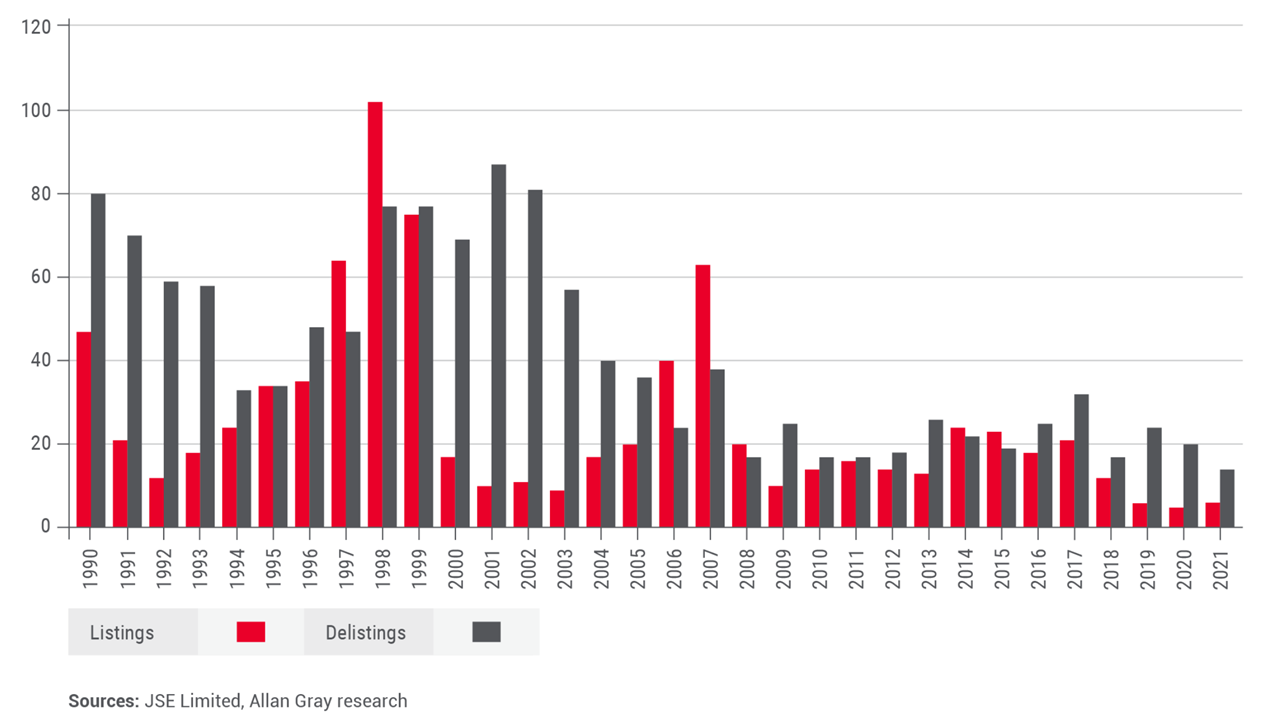
\includegraphics{delist.png}
\caption{Number of New Listings and Delistings}
\end{figure}

A (IOL 2022) busines report noted that the number of delistings was
increasing, with more than one in 10 local listed companies expected to
delist. South Africa was in a seven-year losing streak, averaging 25
company delistings per year, and this trend was accelerating, with 18
companies already having delisted that year and another 14 delisting
processes underway. There was public concern over the future of the JSE,
with social media posts highlighting the ongoing delistings, including
Massmart, Grindrod Shipping, and Rebosis Property Fund. Recenty,
(Bloomberg 2023) reported that the FTSE/JSE Africa All Share Index
currently features 136 companies, down from 165 in 2012, due to onerous
regulatory and funding conditions. The JSE has proposed changes to its
framework to attract more listings, while A2X, a competitor stock
exchange, expects to double its number of listings and increase its
market share in the coming year by offering a more attractive option of
raising capital.

The decreasing number of listed companies on the JSE is causing alarm,
as it not only reflects a weaker market but also raises questions about
the future of the exchange. Some firms may have decided to delist due to
reasons such as a preference to become a private company, a merger or
acquisition by another firm, consolidation, financial struggles, or
failure to comply with listing regulations. In the past three years,
well-known companies like Adapt IT, Alaris, Huge Group, Telemasters,
Massmart, Grindrod Shipping, and Rebosis Property Fund have delisted.
The COVID-19 pandemic has further intensified the global trend of
delisting, and the JSE is facing increased competition from alternative
exchanges such as A2X, which presents itself as a more appealing option
for companies looking to raise capital both inside and outside of South
Africa. The decline in delistings from the JSE is a significant matter
of concern that demands attention and action to secure the stability and
future growth of the exchange. The JSE is predominantly an institutional
market with limited participation from retail customers and has been
criticized for its lack of deep retail customer involvement. Capital
flight from the JSE is anticipated to continue. The JSE CEO, Leila
Fourie, has stated that multiple factors, such as the macro environment
and investor sentiment, are driving the number of listings and
delistings.

In light of a clear increase in the number of delisitings, we
investigate how share prices have moved and build machine learning model
that try and predict the stock prices of 20 randomly selcted pcompanies
still listed on the JSE.

\hypertarget{literature-review}{%
\section{LITERATURE REVIEW}\label{literature-review}}

(Cassim 2000) provide a historical background of the JSE and its
evolution from its inception in 1887 to its current form as a modern
stock exchange. Cassim and Herbst provide an overview of the JSE's
governance structure, its role in the South African economy, and the
types of securities traded on the JSE. This study particularly
highlighted the importance of the JSE as an indicator of the health of
the South African economy and as a source of capital for companies in
South Africa making it an institution of critical importance. In a
similar study Addison and A. Odendaal, (Addison S. 2008), provided a
comprehensive overview of the JSE's history, starting from its
establishment in 1887 to its development in the 20th century. Trace the
evolution of the JSE and its role in the South African economy, focusing
on the exchange's role in supporting the growth of new industries and
providing capital for businesses, the article examined the JSE's
innovations and how they have contributed to its growth and development.
They discussed the introduction of new technologies, such as electronic
trading systems, and the creation of new financial products, such as
derivatives, which have enabled the JSE to compete with other leading
stock exchanges in the world. The article highlighted the challenges
faced by the JSE, including political and economic turmoil, and how the
exchange has adapted to overcome these challenges. The authors concluded
that the JSE has been a leading player in the financial industry,
consistently adapting to changes in the economy and technology to
maintain its position as one of the leading stock exchanges in Africa.
(McDonald 2006), studied the Johannesburg Stock Exchange (JSE) and its
listings in the post-apartheid era. The study provided a historical
background of the JSE, its role in the South African economy, and its
evolution in the post-apartheid era. With an overview of the JSE's
governance structure, its listing requirements, and the types of
securities traded on the JSE, the article consequently highlighted the
impact of the post-apartheid political and economic reforms on the JSE
and its listings. The increased foreign investment in the JSE, and the
growth of new industries and companies listed on the exchange were
discussed as well as the challenges facing the JSE and its listings,
including increased competition from other stock exchanges and the need
for further economic and political reforms. (McDonald 2006), argued that
the JSE had the potential to play a significant role in the growth and
development of the South African economy, and that continued reforms
where necessary to ensure its continued success. (Al-Hawari 2010),
demonstrated that delisting from the Johannesburg Stock Exchange can
have significant impact on shareholder wealth and stock prices. They
provided evidence on the phenomenon of delisting in emerging markets,
specifically the Johannesburg Stock Exchange (JSE) and examined the
reasons for delisting and the impact of delisting on firm value. The
authors used a sample of delisted firms from the JSE for the period from
1997 to 2007. The results of the study show that the main reasons for
delisting from the JSE are financial distress, management decisions, and
mergers and acquisitions. The results also indicate that delisted firms
experience a decline in firm value, and that the decline in firm value
is more pronounced for firms that delist due to financial distress. The
results of the study are relevant for investors, regulators, and policy
makers in emerging markets. Roy, et al, (Roy 2010), study the liquidity
and market quality of the Johannesburg Stock Exchange (JSE). They
analyzed the liquidity and market quality of the JSE over a period of
ten years (1997-2006) and compared the results with other major stock
exchanges around the world. The authors find that the liquidity of the
JSE is generally good, but there is a considerable amount of illiquidity
in the market, particularly in the smaller stocks. They also find that
the market quality of the JSE is lower than that of other major stock
exchanges, due to a high degree of market manipulation, and the absence
of regulations to prevent insider trading and other forms of market
abuse. The authors suggested that the JSE should implement measures to
improve market quality, such as increasing transparency, and
strengthening regulations to prevent market abuse. They also recommend
that the JSE should invest in new technologies, such as electronic
trading systems, to improve the efficiency and competitiveness of the
exchange.

(Chutta 2015), The authors investigate the causes and consequences of
delistings from the Johannesburg Stock Exchange (JSE). The study uses a
sample of 50 companies that delisted from the JSE between 2006 and 2011
and compares them to a control sample of firms that remained listed
during the same period. The results suggest that delistings are
associated with lower liquidity, higher leverage, and lower
profitability compared to firms that remain listed. The authors conclude
that delisting is a negative outcome for both firms and investors and
that regulators should consider policies that support the continued
listing of firms on stock exchanges.

According to Hugo and Chen, (Hugo 2017), the determinants of delisting
from the Johannesburg Stock Exchange include various financial and
non-financial factors such as profitability, liquidity, and size. The
study examines the factors that lead firms to delist from the
Johannesburg Stock Exchange (JSE). The authors use a panel data set of
listed firms on the JSE over a period of 21 years to investigate the
determinants of delistings. They find that firm-specific factors such as
financial performance, size, and age, as well as market-wide factors
such as macroeconomic conditions, play a significant role in the
likelihood of delisting. The authors conclude that their findings
provide important insights for policymakers and regulators looking to
improve the functioning of stock exchanges in emerging markets. (Ntusi
2019), focus on the impact of delistings on shareholder wealth in the
Johannesburg Stock Exchange (JSE). The authors used event study
methodology to examine the impact of delistings announcements on
shareholder wealth around the event. The results suggest that delistings
announcements have a negative impact on shareholder wealth, and the
magnitude of the effect is higher for smaller firms. The findings have
implications for regulators and policymakers, suggesting the need for
increased monitoring of delistings to protect the interests of small
shareholders.

(Magagula 2020), employed a sample of 25 firms delisted from the JSE
between 2013 and 2016 and uses event study methodology to examine the
stock prices of these firms both prior to and after delisting. The
results suggest that delisting has a negative impact on stock prices,
and the magnitude of this effect is influenced by the reasons for
delisting and the characteristics of the firms involved. The authors
conclude that regulators should be mindful of the negative effects of
delisting and work to ensure that such events are managed in a manner
that minimizes harm to stakeholders.

\hypertarget{methodology}{%
\section{METHODOLOGY}\label{methodology}}

\hypertarget{data-issues}{%
\subsection{DATA ISSUES}\label{data-issues}}

The R code is used to retrieve stock price data for 20 different
companies listed on the JSE (Johannesburg Stock Exchange). The data
includes the volume of stocks, open, high, low, close, and adjusted
prices. The relevant libraries are loaded and the BatchGetSymbols
function is used to retrieve the stock prices from January 2016 to the
current date with a monthly frequency. The returned data is stored in a
data.table called stocks\_data and ordered by ticker and ref.date. The
tickers for these 20 companies include ``HAR'', ``SNT'', ``STX'',
``TFG'', ``BHP'', ``SAB'', ``BTI'', ``CFR'', ``AMS'', ``MTN'', ``VOD'',
``CPI'', ``SOL'', ``KIO'', ``ABG'',``SHP'',``SLM'', ``IMP'', ``SSW'',
``MEI'', ``REM'' and represent firms such as Harman International
Industries, Sanlam, Seagate Technology, The Foschini Group, BHP Group,
British American Tobacco, Compagnie Financière Richemont, Amsterdam
Molecular Therapeutics, MTN Group, Vodafone Group, Cape plc, Solaredge
Technologies, Kerry Group, African Rainbow Minerals, Shoprite Holdings,
Standard Life Aberdeen, Impala Platinum Holdings, Seaspan Corporation,
Metair Investments, and Rand Merchant Insurance Holdings.

\hypertarget{data-properties}{%
\subsection{DATA PROPERTIES}\label{data-properties}}

We perform unit root tests on all 20 time series data sets, focusing on
the closing stock prices which we will use in our analysis. We use the
Augmented Dickey Fuller. The null hypothesis for the Augmented
Dickey-Fuller (ADF) unit root test is that the time series has a unit
root, meaning it is non-stationary. In other words, the hypothesis is
that the time series has a trend and there is a systematic pattern to
its behavior that cannot be explained by random fluctuations. The
alternative hypothesis is that the time series is stationary, meaning it
has a constant mean, variance, and autocorrelation structure. The goal
of the ADF test is to determine whether the null hypothesis can be
rejected based on the observed data. If the p-value of the test is less
than 5\%, the null hypothesis is rejected and the time series is
considered to be stationary. If the p-value is greater than the
significance level, then the null hypothesis cannot be rejected and the
time series is considered to have a unit root and be non-stationary. We
use a for-loop to iterate over all stocks and get the following results:

\begin{longtable}[]{@{}lccc@{}}
\caption{Unit Root Test Results}\tabularnewline
\toprule()
ticker & test & statistic & p.value \\
\midrule()
\endfirsthead
\toprule()
ticker & test & statistic & p.value \\
\midrule()
\endhead
HAR & ADF & -3.681082 & 0.0249348 \\
SNT & ADF & -3.681082 & 0.0249348 \\
STX & ADF & -3.681082 & 0.0249348 \\
TFG & ADF & -3.681082 & 0.0249348 \\
BHP & ADF & -3.681082 & 0.0249348 \\
SAB & ADF & -3.681082 & 0.0249348 \\
BTI & ADF & -3.681082 & 0.0249348 \\
CFR & ADF & -3.681082 & 0.0249348 \\
AMS & ADF & -3.681082 & 0.0249348 \\
MTN & ADF & -3.681082 & 0.0249348 \\
VOD & ADF & -3.681082 & 0.0249348 \\
CPI & ADF & -3.681082 & 0.0249348 \\
SOL & ADF & -3.681082 & 0.0249348 \\
KIO & ADF & -3.681082 & 0.0249348 \\
ABG & ADF & -3.681082 & 0.0249348 \\
SHP & ADF & -3.681082 & 0.0249348 \\
SLM & ADF & -3.681082 & 0.0249348 \\
IMP & ADF & -3.681082 & 0.0249348 \\
SSW & ADF & -3.681082 & 0.0249348 \\
MEI & ADF & -3.681082 & 0.0249348 \\
REM & ADF & -3.681082 & 0.0249348 \\
\bottomrule()
\end{longtable}

The time series's for all stocks have no unit roots and we conclude that
they are stationary.

\hypertarget{variable-description}{%
\subsection{VARIABLE DESCRIPTION}\label{variable-description}}

The main variable for this study is the closing stock price. We conduct
a technical analysis which focuses only on price and does not consider a
lot of other values like net profits, market sentiment, amount invested
etc. This is common practice in univariate time series models where by
the behavior of one particular time series is tacked over time and its
relationship to its lags is analyzed. Univariate time series models
usually consider the lags of the variable, known as the autoregressive
part, as well as the lags of the error term, known as the moving average
part. These are known as ARMA(p,q) models where p is number of variable
lags and q the number of error lags. Should the series be
none-stationary, a differencing parameter, d, is added to have an
ARIMA(p,d,q) model. This is the Box-Jenkins approach and we expect the
movement of these stocks to be random thought to an extent predictable.
In light of increased delistings, a fall in stock prices in future is
likely.

\hypertarget{model-selection-and-specification}{%
\subsection{MODEL SELECTION AND
SPECIFICATION}\label{model-selection-and-specification}}

The Box-Jenkins approach is a time series modeling and forecasting
method that involves a series of steps to identify the best model for a
given data set, including data collection and analysis, model
identification, estimation, diagnosis, and forecasting. It is a flexible
and robust method for time series analysis and can be applied to data
sets with trends, seasonality, and autocorrelation. However, it requires
a good understanding of statistical techniques and modeling, and the
process can be complex: (Box 1976)

A technical analysis is done on twenty top performing comapnies on the
JSE. Folowing the Box-Jenkins approach, we first implement an Auto-ARIMA
model which, according to (Hyndman 2008), is a time series forecasting
method that combines both ARIMA and machine learning techniques. The
goal of Auto-ARIMA is to automatically determine the best ARIMA model
parameters for a given time series, and to provide accurate forecasting
results; Auto-ARIMA works by first performing an initial analysis of the
time series data to identify trends, seasonality, and other patterns.
Based on this analysis, the method then tests various ARIMA models and
chooses the one that provides the best fit for the data. Auto-ARIMA also
includes a stepwise model selection process, where it tries different
combinations of p, d, and q parameters until it finds the optimal
combination that minimizes the prediction error.

An ARIMA(p,d,q) can be specified as:

\[y_t = c + {\phi}_1y_{t-1} + {\phi}_2y_{t-2}+ .... +{\phi}_py_{t-p} - {\theta}_1e_{t-1} - {\theta}_2e_{t-2} - ... - {\theta}_qe_{t-q} + {\theta}_t\]

where \(y_t\) is the current observation, \(c\) is a constant term,
\({\phi}_1\) to \({\phi}_q\) are the autoregressive coefficients,
\({\theta}_1\) to \({\theta}_q\) are the moving average coefficients,
\(e_t\) is the residual (error) term and the parameters ``p'', ``d'' and
``q'' in the ARIMA model represent the order of the AR component, the
degree of differencing required, and the order of the MA component,
respectively.

The auto.arima() function in the R package ``forecast'' is used to
automatically select the optimal ARIMA model based on the Akaike
information criterion (AIC) and Bayesian information criterion (BIC).
Once the ARIMA model has been fit to the time series data, it is used to
generate forecasts for future observations, which can be adjusted for
any exogenous variables by specifying them as the xreg argument in the
forecast() function.

We then use the Recurrent Neural Network (RNN) on the same dataset.
(Hochreiter 1997) explained the RNN is a type of deep learning neural
network that is designed to process sequential data. The network is
trained to recognize patterns in sequences of data, and it can use these
patterns to make predictions. RNNs are particularly well-suited to time
series forecasting, as they can capture and retaining information about
the past to inform future predictions. In an RNN, the hidden state of
the network is updated at each time step based on both the current input
and the previous hidden state. This allows the network to build a rich
internal representation of the sequence, and to use this representation
to make predictions about future events. A simple neural network
representaion is:

\[h_t = \tanh(W_x \times x_t + W_h \times h_{t-1} + b)\]
\[y_t = W_y \times h_t + b_y\]

where \(h_t\) is the hidden state at time \(t\), \(x_t\) is the input at
time \(t\), \(W_x\) is the weight matrix for the input, \(W_h\) is the
weight matrix for the hidden state, \(b\) is the bias vector \(y_t\) is
the output at time \(t\), \(W_y\) is the weight matrix for the output
and \(b_y\) is the bias vector for the output.

RNNs can be used with different types of activation functions, such as
the Long Short-Term Memory (LSTM) or the Gated Recurrent Unit (GRU), to
handle various types of sequences. This code is using the caret library
to perform time series prediction using Recurrent Neural Network (RNN)
model. The data is split into train and test sets for each stock using
createDataPartition and lapply functions. The RNN model is defined in
the rnn\_model function. This function takes the train and test data for
each stock and trains the model using the caret's train function. The
predict function is then used to make predictions on the test data. The
sapply function is used to apply the rnn\_model to each stock. The final
result is stored in the predictions object.

\hypertarget{visualisations}{%
\section{VISUALISATIONS}\label{visualisations}}

The top 20 companies on the JSE as at 11 February 2023 are shown in
Figure 3 in the appendix and these are some of the companies used in our
analysis. Firstly, the graphs show how some for he biggest companies on
the JSE in terms of market capitalization have performed from 2016 to
date have performed. Companies like ABSA (ABG), BHP Group Limited (BHP),
RICHEMONT (CFR), MTN GROUP (MTN ) and SHOPRIT (SHP) show a general
upward trend whilst companies like SANTAM (SNT), VODACOM (VOD), AMPLATS
(AMS) and BATS (BTI) show a persistent downward trend.

\begin{figure}
\centering
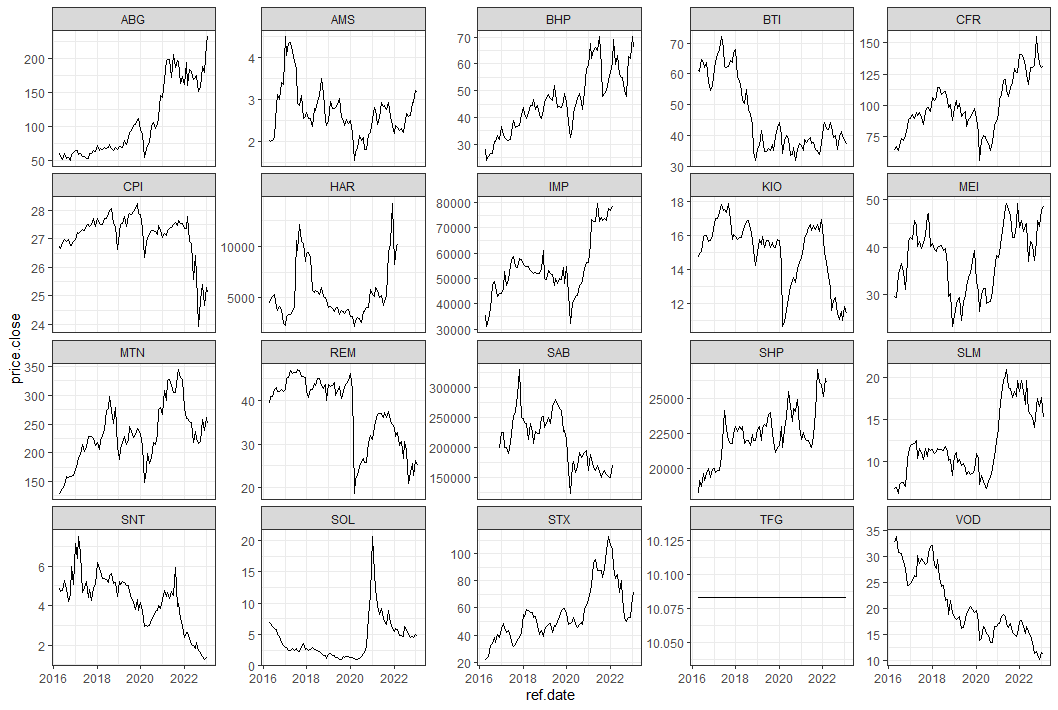
\includegraphics{prices.png}
\caption{Number of New Listings and Delistings}
\end{figure}

The returns for all 20 stocks in this study, as shown in Figure 4 in the
appendix, are mean reverting and hence ARIMA time series models can used
when the stock prices are either differenced or logged.

\hypertarget{data-pre-processing}{%
\subsection{DATA PRE-PROCESSING}\label{data-pre-processing}}

The data pre-processing process involves preparing a time series data
set for analysis and modeling. By focusing on only the ``price.close''
column, the data set is reduced to a single variable that represents the
closing price of a financial instrument (such as a stock or a currency)
at a given time. Next, the data set is split into two parts using the
``caTools'' package: the training set and the test set. The training set
is used to fit the model, while the test set is used to evaluate its
performance. This split is important because it allows the model to be
tested on new, unseen data, which helps to assess its generalization
ability and prevent overfitting. Overfitting occurs when a model is too
closely fit to the training data and performs poorly on new, unseen
data.

\hypertarget{evaluating-the-models-using-the-mse}{%
\section{EVALUATING THE MODELS USING THE
MSE}\label{evaluating-the-models-using-the-mse}}

the Mean Squared Error (MSE) is a commonly used criterion for evaluating
machine learning models and it is the average squared difference between
the predicted values of a model and the actual values of the target
variable. The idea behind MSE is to penalize large errors and reward
models that make small errors. The smaller the MSE, the better the model
is considered to be at making predictions.

The MSE error is given by:

\[MSE = (1\div{N})\times\sum(y_i - \hat{y}_i)^2\] Where \(y_i\) is the
actual value of the target variable for sample \(i\) and \(\hat{y}_i\)
is the predicted value of the target variable for sample \(i\).

The avearge mean square error is used to evaluate the model.

\hypertarget{concluding-remarks}{%
\section{CONCLUDING REMARKS}\label{concluding-remarks}}

Only the prices where considered in this study, whereby future prices
where predicted based on historic prices. These models are informative
and with very small root mean square errors, they seem to good models.
However, more informative models can be done using fundamental analysis,
this implies that more than just the researcher takes into consideration
more than just prices. Using fundamental analysis, machine learning
models such as Artificial Neural Networks (ANNs), Support Vector
Regression (SVR) and Random Forests can be utilized. These methodologies
can be used to predict stock prices by considering a wide range of
factors, such as technical indicators, market sentiment, and news
articles. With more information in the model it is logical to assume we
would get better predictions.

\newpage

\hypertarget{appendix}{%
\section{APPENDIX}\label{appendix}}

\begin{figure}
\centering
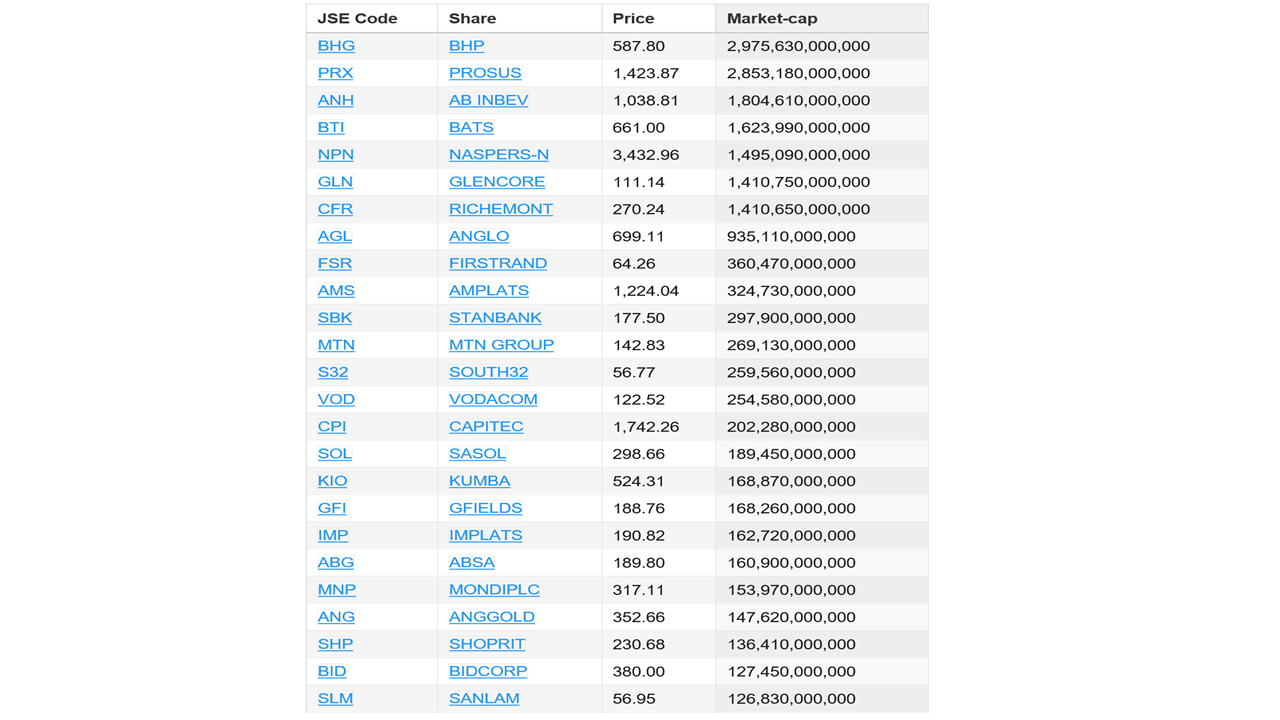
\includegraphics{stockprice.png}
\caption{Number of New Listings and Delistin}
\end{figure}

\begin{figure}
\centering
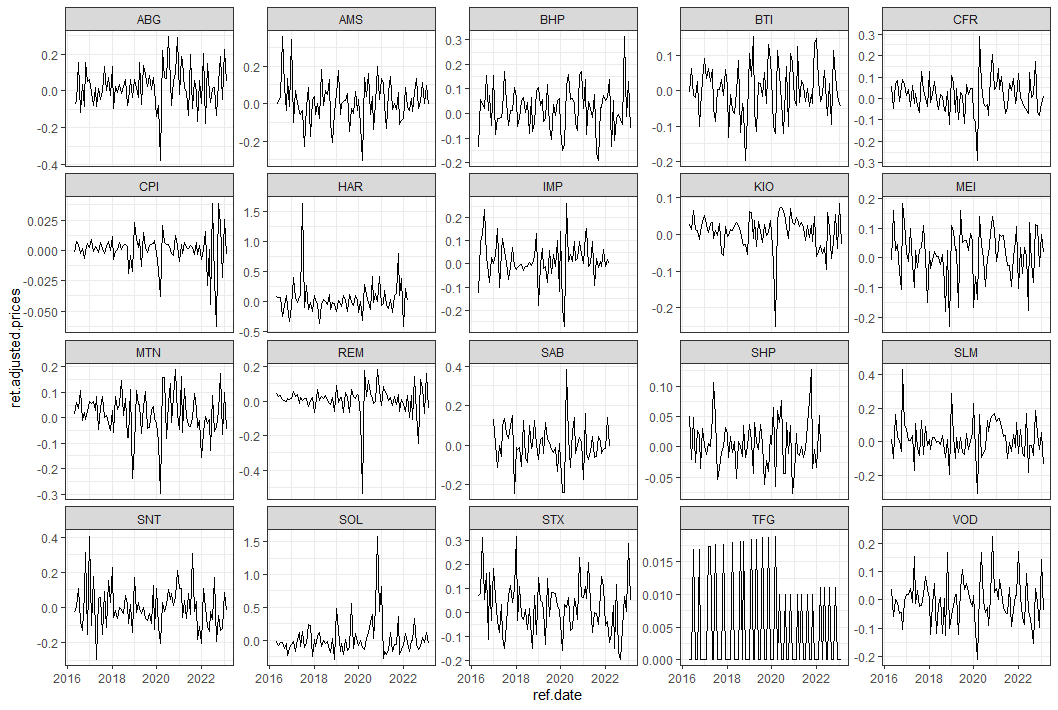
\includegraphics{returns.png}
\caption{Stock Returns}
\end{figure}

\newpage

\hypertarget{references}{%
\section{REFERENCES}\label{references}}

\bibliography{references.bib}

\hypertarget{refs}{}
\begin{CSLReferences}{1}{0}
\leavevmode\vadjust pre{\hypertarget{ref-addison2008hist}{}}%
Addison S., Odendaal A. 2008. {``The Johannesburg Stock Exchange: A
History of Innovation.''} \emph{South African Journal of Economic
History} 23 (1): 1--19.

\leavevmode\vadjust pre{\hypertarget{ref-alhawari2010delisting}{}}%
Al-Hawari, Papke, M. E. 2010. {``Delisting in Emerging Markets: Evidence
from the Johannesburg Stock Exchange.''} \emph{Journal of Emerging
Market Finance} 9 (3): 299--323.

\leavevmode\vadjust pre{\hypertarget{ref-Bloomberg2023}{}}%
Bloomberg. 2023. {``No End in Sight for South Africa's Delisting Trend,
Says A2X CEO.''} 2023.
\url{https://www.engineeringnews.co.za/article/no-end-in-sight-for-south-africas-delisting-trend-says-a2x-ceo-2023-01-20}.

\leavevmode\vadjust pre{\hypertarget{ref-box1976}{}}%
Box, \& Jenkins, G. E. 1976. {``Time Series Analysis: Forecasting and
Control.''} \emph{San Francisco: Holden-Day}.

\leavevmode\vadjust pre{\hypertarget{ref-BusinessTech2021}{}}%
BusinessTech. 2021. {``South Africa's Shrinking JSE - Investors Explain
What's Going On.''} 2021.
\url{https://businesstech.co.za/news/finance/467553/south-africas-shrinking-jse-investors-explain-whats-going-on/}.

\leavevmode\vadjust pre{\hypertarget{ref-cassim2000jse}{}}%
Cassim, \& Herbst, M. L. 2000. {``The Johannesburg Stock Exchange: An
Overview.''} \emph{Journal of African Business} 1 (1): 1--18.

\leavevmode\vadjust pre{\hypertarget{ref-chutta2015delist}{}}%
Chutta, Dimitropoulos, K. S. 2015. {``Delistings from the Johannesburg
Stock Exchange: Causes, Characteristics and Consequences.''}
\emph{Journal of African Business} 16 (4): 333--54.

\leavevmode\vadjust pre{\hypertarget{ref-Hochreiter1997long}{}}%
Hochreiter, \& Schmidhube, S. 1997. {``Long Short-Term Memory.''}
\emph{Neural Computation} 9 (8): 1735--80.

\leavevmode\vadjust pre{\hypertarget{ref-hugo2017determ}{}}%
Hugo, \& Chen, D. L. 2017. {``The Determinants of Delistings from the
Johannesburg Stock Exchange.''} \emph{Journal of Financial Regulation
and Compliance} 25 (4): 338--58.

\leavevmode\vadjust pre{\hypertarget{ref-hyndaman2008auto}{}}%
Hyndman, \& Khandakar, R. J. 2008. {``Automatic Time Series Forecasting:
The Forecast Package for r.''} \emph{Journal of Statistical Software} 26
(3): 1--22.

\leavevmode\vadjust pre{\hypertarget{ref-IOL2022}{}}%
IOL. 2022. {``JSE Is Bleeding: One-in-10 Local Listed Companies Forecast
to Delist This Year.''} 2022.
\url{https://www.iol.co.za/business-report/companies/jse-is-bleeding-one-in-10-local-listed-companies-forecast-to-delist-this-year-dbc7f63d-1819-4137-b216-044756c09cfd}.

\leavevmode\vadjust pre{\hypertarget{ref-magagula2020conseq}{}}%
Magagula, \& Moemi, N. I. 2020. {``The Consequences of Delisting on
Stock Prices: Evidence from the Johannesburg Stock Exchange.''}
\emph{African Journal of Accounting, Auditing and Finance} 9 (1):
51--63.

\leavevmode\vadjust pre{\hypertarget{ref-mcdonald2006post}{}}%
McDonald, D. G. 2006. {``Post-Apartheid South Africa: A Study of the
Johannesburg Stock Exchange and Its Listings.''} \emph{Journal of
Transnational Management} 11 (3): 175--95.

\leavevmode\vadjust pre{\hypertarget{ref-ntusi2019impact}{}}%
Ntusi, \& Moemi, C. Z. 2019. {``The Impact of Delistings on Shareholder
Wealth: Evidence from the Johannesburg Stock Exchange.''} \emph{Journal
of Applied Economics and Business Research} 8 (4): 249--66.

\leavevmode\vadjust pre{\hypertarget{ref-roy2010liq}{}}%
Roy, Longstaff, T. K. 2010. {``Liquidity and Market Quality in the
Johannesburg Stock Exchange.''} \emph{Journal of Financial
Intermediation} 19 (2): 246--65.

\end{CSLReferences}

\end{document}
